\section{Diskussion}
\label{sec:Diskussion}

% theoretische werte µ: 69.351 für blei, 50.544 für zink

Die theoretisch ermittelten Werte für die Compton-Absorptionskoeffizienten lassen sich aus \eqref{eqlig2} ermitteln. Unter Benutzung von \eqref{eqliq} und den Werten aus \autoref{tabelle}, ergeben sich die theoretischen Werte
\begin{eqnarray}
  \mu_{Pb} &=& 69,43  \mathrm{m^-1}\ und \nonumber \\
  \mu_{Zn} &=& 22,78  \mathrm{m^-1}, \nonumber 
\end{eqnarray}
die sich mit den experimentiell bestimmten 
\begin{eqnarray}
  \mu_{Pb} &=&   \pm  \,  \mathrm{m^-1} \nonumber \\
  \mu_{Zn} &=&   \pm  \,  \mathrm{m^-1} \nonumber 
\end{eqnarray}
vergleichen lassen.
\begin{table}[H]
 \centering
 \caption{Theoretische Werte für Zink und Blei \cite{2} \cite{3}.}
 \begin{tabular}{l|l|l|l}
 & z & M/$\frac{\textrm{mol}}{g}$ & $\rho$/$\frac{\textrm{cm}^3}{g}$\\\hline
 Blei & 82 & 207,2 & 11,34\\
 Zink & 30 & 65 & 7,14\\\hline
 \end{tabular}
\end{table}
Die Werte aus dem Experiment zeigen eine Abweichung von
\begin{eqnarray}
  \eta_{Pb} &=& 27,1 \ \% \nonumber \\
  \eta_{Zn} &=& 47,1 \ \% \nonumber 
\end{eqnarray}
Die Abweichungen können aus Überlagerungen des Compton-Effekts und des Photo-Effekts folgen.\\
Der theoretische Wert der maximal Energie der Beta-Strahlung von Technetium liegt bei $E=0,294$ MeV. Wird dieser mit dem experimentellen Wert $E_{exp}=0,19$ MeV verglichen, ergibt sich eine Abweichung von 
\begin{equation*}
  \eta_{E}=54,7 \ \%
\end{equation*}
die sehr groß ist. Das kann aus der Ausgleichsrechnung folgen. 

\section{Anhang}
\label{sec:anhang}

\begin{figure}[H]
  \centering
  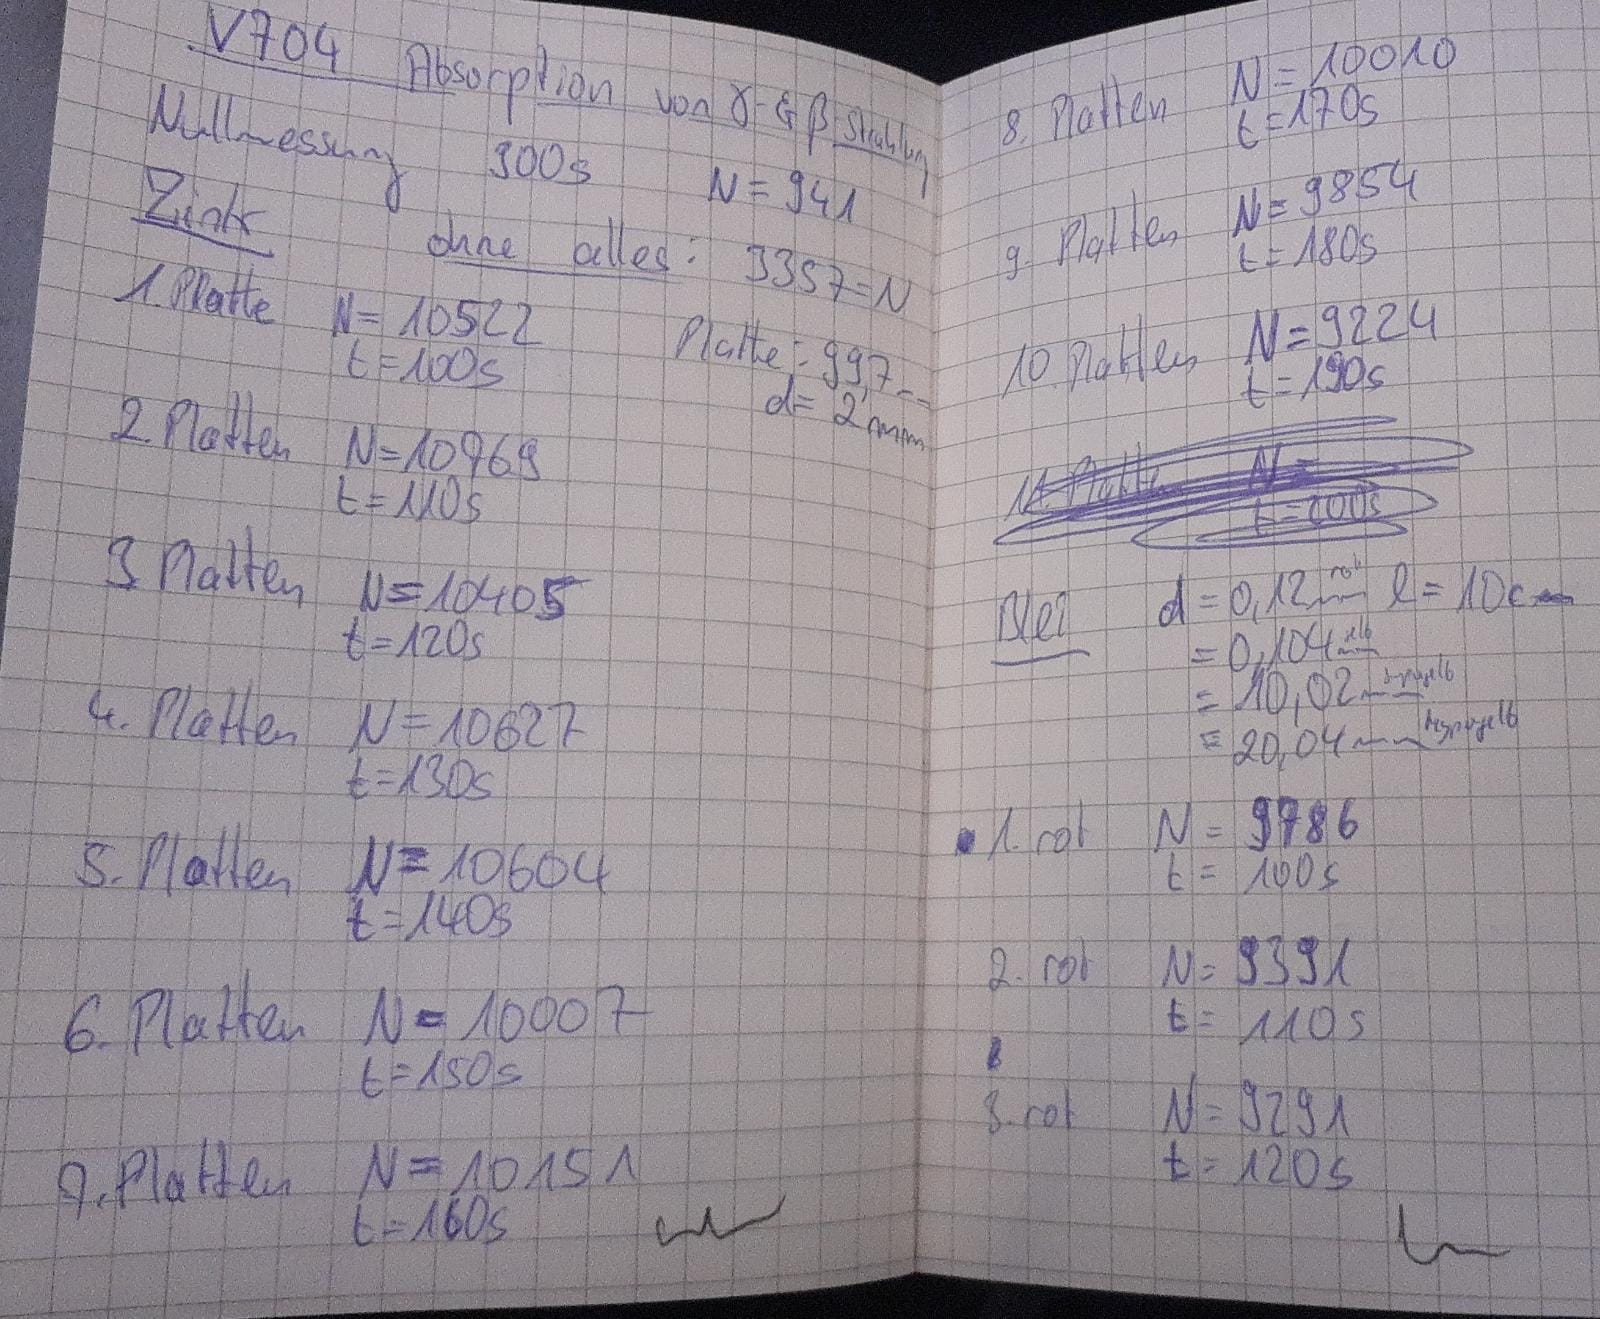
\includegraphics{content/mess1.jpg}
  \caption{Die aufgenommenen Messwerte.}
  \label{fig:mess1}
\end{figure}
\begin{figure}[H]
  \centering
  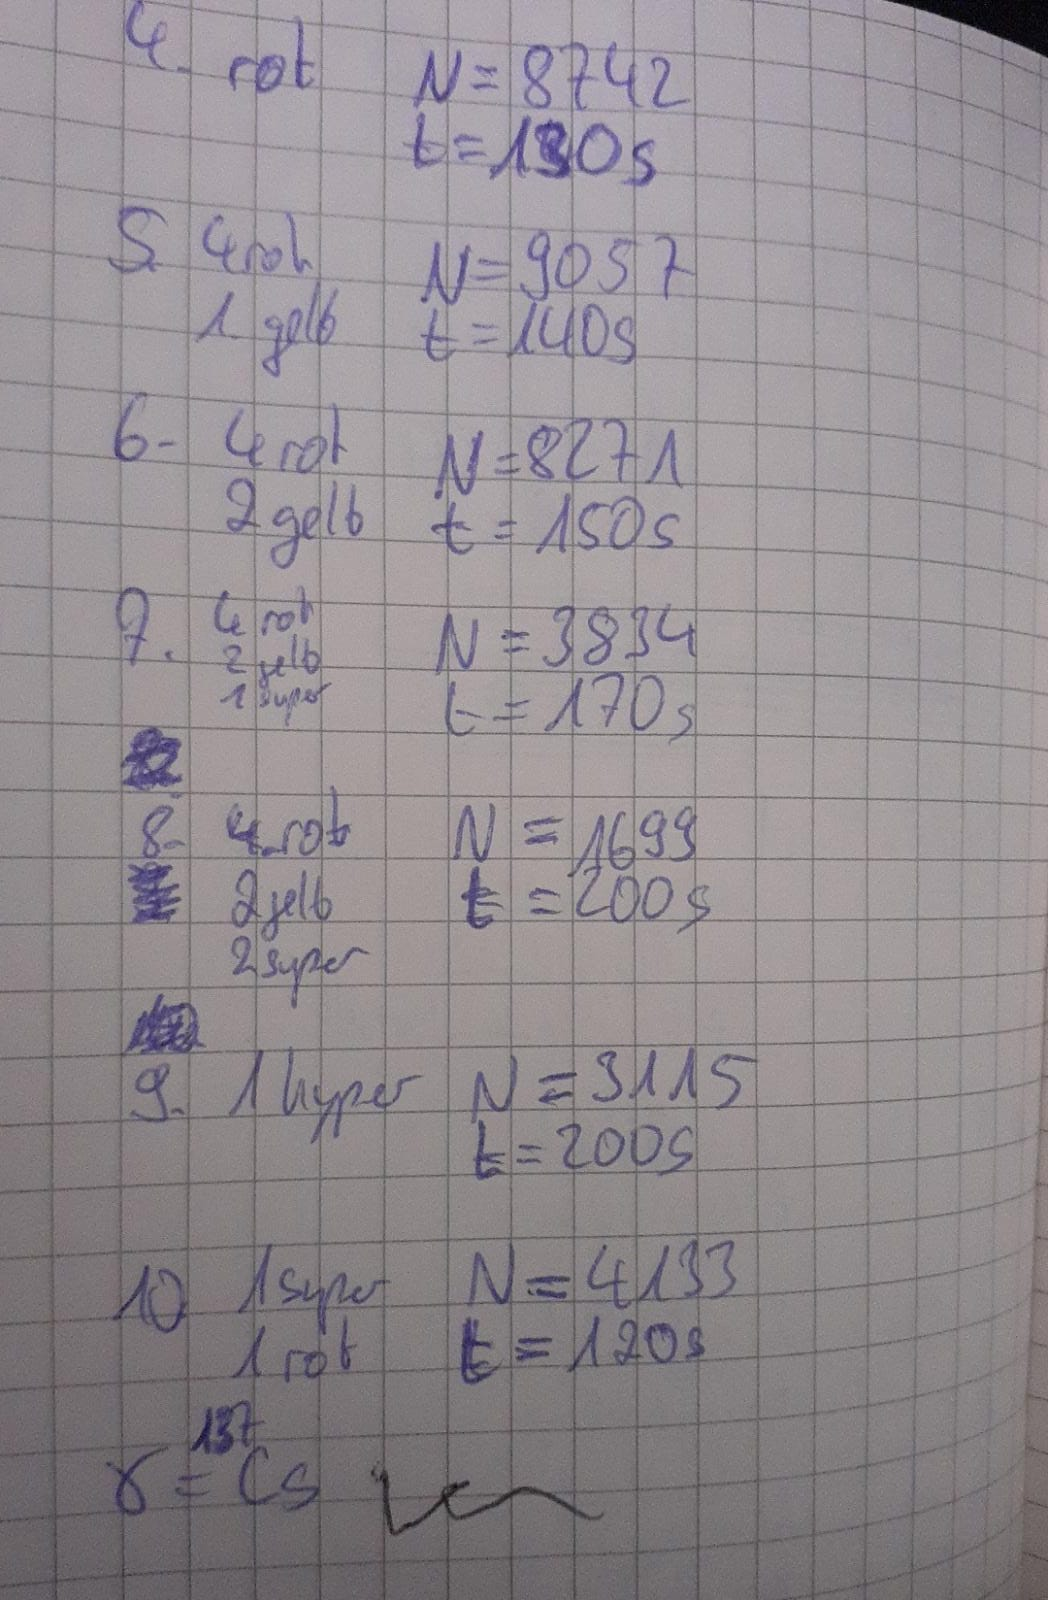
\includegraphics{content/mess2.jpg}
  \caption{Die aufgenommenen Messwerte.}
  \label{fig:mess2}
\end{figure}
\begin{figure}[H]
  \centering
  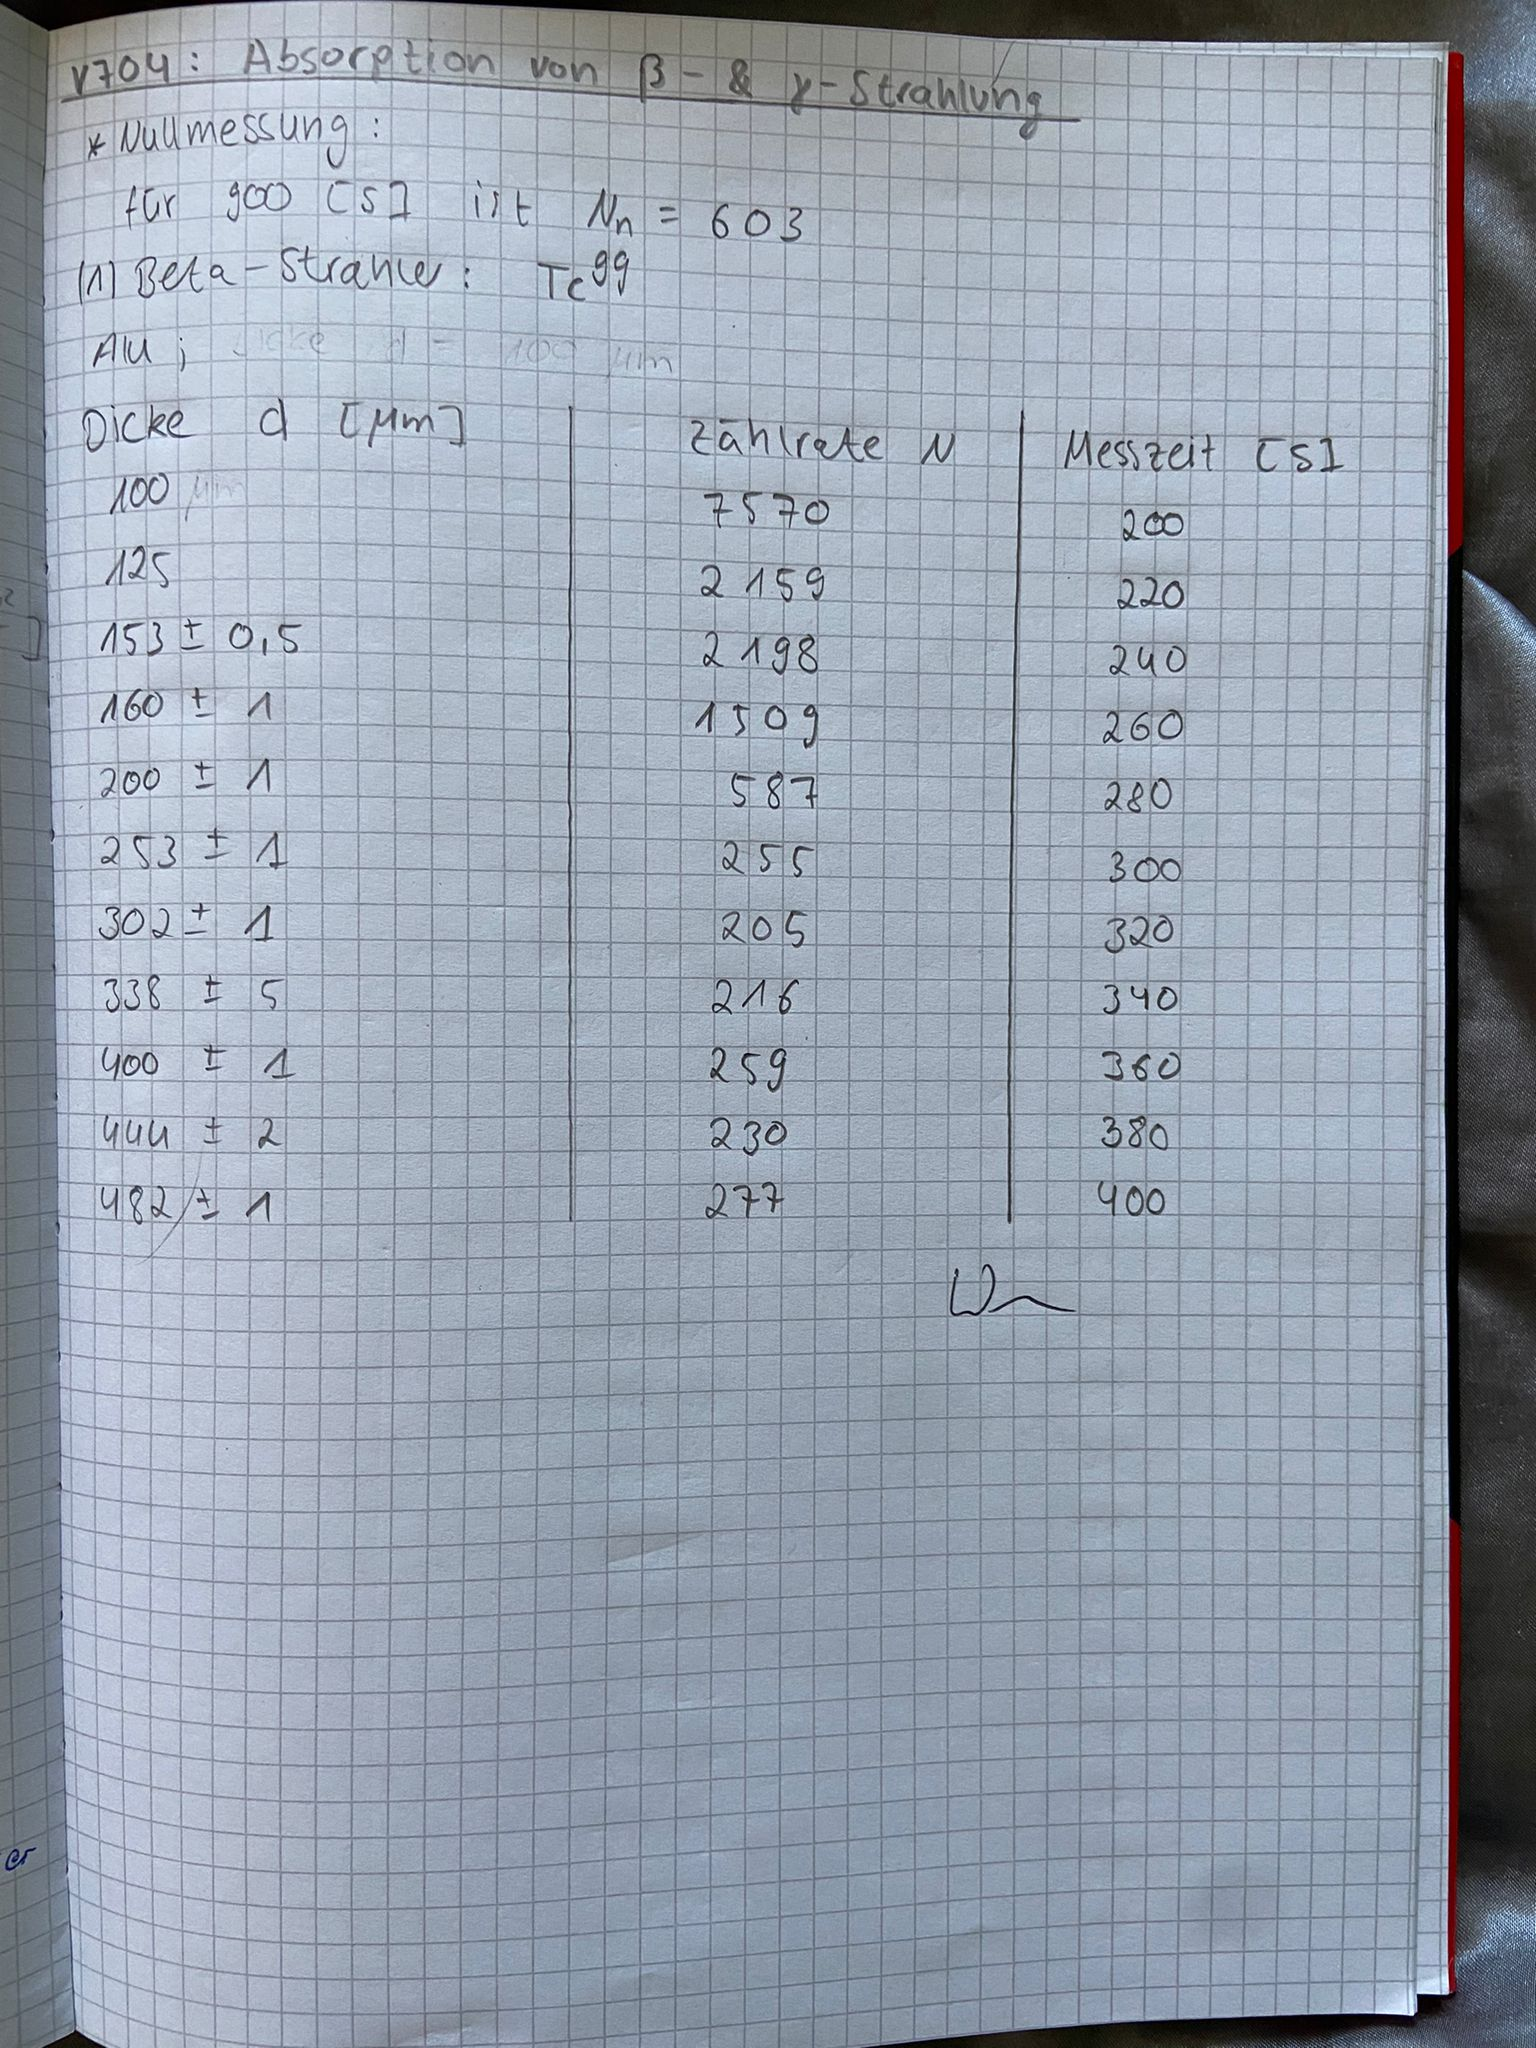
\includegraphics{content/messbeta.jpeg}
  \caption{Die aufgenommenen Messwerte.}
  \label{fig:messbeta}
\end{figure}
